\documentclass[12pt,a4paper]{article}
\usepackage{amsmath}
\usepackage{amssymb}
\usepackage{graphicx}
\usepackage{tikz}
\usepackage{float}
\usepackage{hyperref}
\usepackage{listings}
\usepackage{color}
\usepackage{algorithm}
\usepackage{algorithmic}

\title{Understanding Uniform B-Splines: Mathematical Foundation and Intuitive Explanation}
\author{Technical Documentation}
\date{\today}

\begin{document}

\maketitle

\tableofcontents
\newpage

\section{Introduction: What is a B-Spline?}

\subsection{The Simple Explanation}

Imagine you're drawing a smooth curve through a series of points, but instead of the curve passing directly through each point, you want it to be ``influenced'' by these points while remaining smooth. This is what B-splines do!

Think of it like this:
\begin{itemize}
    \item You have a rubber band that you want to shape into a smooth curve
    \item You place magnets (control points) near the rubber band
    \item The rubber band curves smoothly, attracted by the magnets but not necessarily touching them
    \item The final shape is smooth and predictable
\end{itemize}

\subsection{Why Use B-Splines for Robot Trajectories?}

B-splines are perfect for robot path planning because:
\begin{enumerate}
    \item \textbf{Smoothness}: They guarantee smooth velocity and acceleration profiles
    \item \textbf{Local Control}: Moving one control point only affects a small portion of the curve
    \item \textbf{Computational Efficiency}: Fast to evaluate and modify
    \item \textbf{Convex Hull Property}: The curve stays within the boundary of control points
\end{enumerate}

\section{Mathematical Foundation}

\subsection{Basic Definition}

A B-spline curve of degree $p$ is defined as:

\begin{equation}
    \mathbf{C}(u) = \sum_{i=0}^{n} N_{i,p}(u) \mathbf{P}_i
\end{equation}

where:
\begin{itemize}
    \item $\mathbf{C}(u)$ is the curve at parameter $u$
    \item $\mathbf{P}_i$ are the control points (the ``magnets'' in our analogy)
    \item $N_{i,p}(u)$ are the B-spline basis functions (the ``influence'' of each magnet)
    \item $n+1$ is the number of control points
    \item $p$ is the degree of the curve (we use $p=3$ for cubic B-splines)
\end{itemize}

\subsection{The Cox-de Boor Recursion Formula}

The basis functions $N_{i,p}(u)$ are computed recursively using the Cox-de Boor formula:

\begin{align}
    N_{i,0}(u) &= \begin{cases}
        1 & \text{if } t_i \leq u < t_{i+1} \\
        0 & \text{otherwise}
    \end{cases} \\[10pt]
    N_{i,p}(u) &= \frac{u - t_i}{t_{i+p} - t_i} N_{i,p-1}(u) + \frac{t_{i+p+1} - u}{t_{i+p+1} - t_{i+1}} N_{i+1,p-1}(u)
\end{align}

where $\mathbf{t} = [t_0, t_1, ..., t_m]$ is the knot vector.

\subsection{Uniform B-Splines: The Special Case}

In a \textbf{uniform} B-spline, the knots are equally spaced:
\begin{equation}
    t_{i+1} - t_i = \Delta t \quad \text{(constant for all } i\text{)}
\end{equation}

This makes the math simpler and the curve more predictable!

\section{Intuitive Understanding}

\subsection{The Blending Concept}

Think of B-splines as a \textbf{weighted average} of control points:

\begin{center}
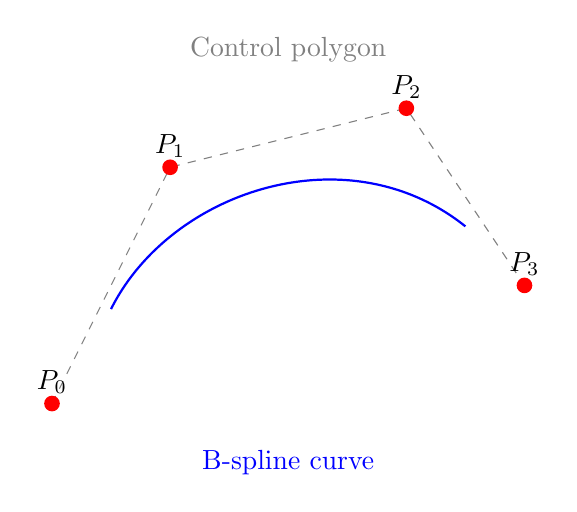
\begin{tikzpicture}[scale=1.5]
    % Control points
    \coordinate (P0) at (0,0);
    \coordinate (P1) at (1,2);
    \coordinate (P2) at (3,2.5);
    \coordinate (P3) at (4,1);
    
    % Draw control polygon
    \draw[gray,dashed] (P0) -- (P1) -- (P2) -- (P3);
    
    % Draw control points
    \foreach \i in {0,1,2,3} {
        \node[circle,fill=red,inner sep=2pt] at (P\i) {};
        \node[above] at (P\i) {$P_\i$};
    }
    
    % Draw B-spline curve (approximation)
    \draw[blue,thick] (0.5,0.8) .. controls (1,1.8) and (2.5,2.3) .. (3.5,1.5);
    
    % Label
    \node[blue] at (2,-0.5) {B-spline curve};
    \node[gray] at (2,3) {Control polygon};
\end{tikzpicture}
\end{center}

At any point on the curve:
\begin{itemize}
    \item The curve is a blend of nearby control points
    \item Each control point has a ``region of influence''
    \item The influence smoothly fades in and out
\end{itemize}

\subsection{Why Cubic (Degree 3)?}

We use cubic B-splines because they provide:
\begin{itemize}
    \item $C^2$ continuity: Smooth position, velocity, AND acceleration
    \item Minimum curvature: The smoothest possible path
    \item Local support: Each control point affects only 4 knot spans
\end{itemize}

\section{Algorithm Implementation}

\subsection{Evaluating a Point on the Curve}

Here's the step-by-step process:

\begin{algorithm}
\caption{Evaluate B-Spline at Parameter $u$}
\begin{algorithmic}
\STATE \textbf{Input:} Parameter $u$, control points $\mathbf{P}$, knot vector $\mathbf{t}$, degree $p$
\STATE \textbf{Output:} Point on curve $\mathbf{C}(u)$
\STATE
\STATE 1. Find knot span: Find $i$ such that $t_i \leq u < t_{i+1}$
\STATE 2. Compute basis functions $N_{j,p}(u)$ for $j = i-p, ..., i$
\STATE 3. Compute curve point: $\mathbf{C}(u) = \sum_{j=i-p}^{i} N_{j,p}(u) \mathbf{P}_j$
\end{algorithmic}
\end{algorithm}

\subsection{Practical Example: Robot Path}

Consider a robot moving in a square pattern:

\begin{enumerate}
    \item \textbf{Waypoints}: $(0,0) \rightarrow (1,0) \rightarrow (1,1) \rightarrow (0,1) \rightarrow (0,0)$
    \item \textbf{Control Points}: Generated from waypoints with corner handling
    \item \textbf{Knot Vector}: Uniform spacing, e.g., $[0, 0.1, 0.2, 0.3, ...]$
    \item \textbf{Result}: Smooth curve that rounds the corners
\end{enumerate}

\section{Key Properties for Robotics}

\subsection{Velocity Profile}

The velocity along the B-spline is the first derivative:
\begin{equation}
    \mathbf{V}(u) = \frac{d\mathbf{C}(u)}{du} = \sum_{i=0}^{n-1} N_{i,p-1}(u) \cdot p \cdot \frac{\mathbf{P}_{i+1} - \mathbf{P}_i}{t_{i+p+1} - t_{i+1}}
\end{equation}

\subsection{Acceleration Profile}

The acceleration is the second derivative:
\begin{equation}
    \mathbf{A}(u) = \frac{d^2\mathbf{C}(u)}{du^2}
\end{equation}

For cubic B-splines, this is always continuous!

\subsection{Arc Length Parameterization}

For robot control, we need to move at constant speed. The arc length from $u_0$ to $u$ is:
\begin{equation}
    s(u) = \int_{u_0}^{u} \left\| \frac{d\mathbf{C}(\tau)}{d\tau} \right\| d\tau
\end{equation}

We pre-compute this and create a mapping: arc length $\leftrightarrow$ parameter $u$.

\section{Simple Numerical Example}

Let's work through a simple 1D example with 4 control points:

\begin{itemize}
    \item Control points: $P_0 = 0$, $P_1 = 1$, $P_2 = 2$, $P_3 = 1$
    \item Degree: $p = 3$ (cubic)
    \item Uniform knots: $[0, 1, 2, 3, 4, 5, 6, 7]$
\end{itemize}

At $u = 3.5$ (middle of the curve):
\begin{enumerate}
    \item Knot span: $i = 3$ (since $3 \leq 3.5 < 4$)
    \item Active control points: $P_0, P_1, P_2, P_3$
    \item Basis functions at $u = 3.5$:
    \begin{align*}
        N_{0,3}(3.5) &= 0.0208 \\
        N_{1,3}(3.5) &= 0.2292 \\
        N_{2,3}(3.5) &= 0.5208 \\
        N_{3,3}(3.5) &= 0.2292
    \end{align*}
    \item Curve point: 
    \begin{equation*}
        C(3.5) = 0.0208 \cdot 0 + 0.2292 \cdot 1 + 0.5208 \cdot 2 + 0.2292 \cdot 1 = 1.5
    \end{equation*}
\end{enumerate}

\section{Advantages for Robot Control}

\subsection{Smooth Motion}
\begin{itemize}
    \item No sudden velocity changes (continuous first derivative)
    \item No sudden acceleration changes (continuous second derivative)
    \item Minimizes mechanical stress on robot motors
\end{itemize}

\subsection{Efficient Computation}
\begin{itemize}
    \item $O(p \cdot d)$ evaluation time where $p$ is degree and $d$ is dimension
    \item Pre-computable arc length tables
    \item Local support means fast updates
\end{itemize}

\subsection{Robust to Noise}
\begin{itemize}
    \item Small errors in control points don't cause large trajectory changes
    \item Natural smoothing of waypoint data
    \item Convex hull property prevents wild oscillations
\end{itemize}

\section{Practical Tips for Implementation}

\subsection{Choosing the Number of Control Points}

\begin{itemize}
    \item Too few: Cannot represent complex paths
    \item Too many: Over-fitting, computational overhead
    \item Rule of thumb: $n = 1.5 \times$ number of waypoints
\end{itemize}

\subsection{Handling Sharp Corners}

For sharp turns (like in a square path):
\begin{enumerate}
    \item Add extra control points near corners
    \item Offset control points slightly from corner vertices
    \item Use lower degree (2) for sharper corners if needed
\end{enumerate}

\subsection{Real-time Replanning}

The EWOK approach allows updating only a few control points:
\begin{itemize}
    \item Keep distant control points fixed
    \item Update only nearby control points based on sensor data
    \item Maintains smoothness while adapting to obstacles
\end{itemize}

\section{Common Pitfalls and Solutions}

\subsection{Problem: Curve doesn't pass through waypoints}
\textbf{Solution}: B-splines approximate, not interpolate. Use interpolating splines or add constraints if exact waypoint passing is required.

\subsection{Problem: Oscillations near constraints}
\textbf{Solution}: Use tension parameters or reduce the degree locally.

\subsection{Problem: Slow evaluation for long paths}
\textbf{Solution}: Use spatial data structures to quickly find the active knot span.

\section{Conclusion}

Uniform B-splines provide an elegant solution for robot trajectory planning:
\begin{itemize}
    \item \textbf{Mathematically}: Well-defined with proven properties
    \item \textbf{Computationally}: Efficient to evaluate and modify
    \item \textbf{Practically}: Smooth, predictable robot motion
    \item \textbf{Intuitively}: Like shaping a flexible ruler with magnetic influence points
\end{itemize}

The key insight is that B-splines give us \textbf{local control with global smoothness} -- exactly what we need for robust robot navigation!

\section{References and Further Reading}

\begin{itemize}
    \item De Boor, C. (1978). \textit{A Practical Guide to Splines}
    \item Piegl, L. \& Tiller, W. (1997). \textit{The NURBS Book}
    \item Usenko, V., et al. (2017). \textit{Real-time trajectory replanning for MAVs using uniform B-splines} (EWOK)
    \item Cox, M.G. (1972). \textit{The numerical evaluation of B-splines}
\end{itemize}

\appendix

\section{Mathematical Proofs}

\subsection{Proof of Partition of Unity}

For B-spline basis functions:
\begin{equation}
    \sum_{i=0}^{n} N_{i,p}(u) = 1 \quad \text{for all } u \in [t_p, t_{n+1}]
\end{equation}

This ensures the curve is a true weighted average.

\subsection{Proof of Convex Hull Property}

Since $N_{i,p}(u) \geq 0$ and $\sum_i N_{i,p}(u) = 1$, the curve point $\mathbf{C}(u)$ is a convex combination of control points, hence lies within their convex hull.

\section{Implementation Code Structure}

\begin{lstlisting}[language=C++, caption=B-Spline Evaluation Pseudocode]
struct BSpline {
    vector<Point> control_points;
    vector<double> knot_vector;
    int degree;
    
    Point evaluate(double u) {
        int span = findKnotSpan(u);
        vector<double> basis = computeBasis(span, u);
        Point result = Point::zero();
        
        for (int i = 0; i <= degree; ++i) {
            result += basis[i] * control_points[span - degree + i];
        }
        return result;
    }
    
    vector<double> computeBasis(int span, double u) {
        // Cox-de Boor recursion
        // Returns basis functions N_{i,p}(u)
    }
};
\end{lstlisting}

\end{document}